\documentclass[a4,10pt]{article}
\usepackage{xparse,av}
\usepackage{epsfig}
\usepackage[colorlinks=true]{hyperref}
\usepackage[latin2]{inputenc}
\usepackage{amsmath,amssymb}
\setlength{\textwidth}{17.5cm}
\setlength{\textheight}{22 cm}
\setlength{\topmargin}{-1cm}
\setlength{\oddsidemargin}{-1cm}
\pagestyle{headings}
\newcommand{\pdd}[1]{\partial_{\textstyle{#1}}}

\begin{document}

\title{WHAMP quick reference (v 1.4)}
\author{A. Vaivads}
\maketitle

\section{\WHAMP\ introduction }

\WHAMP\ calculates the dispersion relation of Waves in Homogeneous Anisotropic Magnetized Plasma. Each plasma component consists of particles with charge $q_{j}$, mass $m_{j}$, density $n_{j}$ and  normalized distribution function $\tilde{f}^{j}(\vv,\vr)$. The phase space density $f^{j}$ can be obtained as $f^j=\tilde{f}^j n^j$.
The general distribution function considered has the form of an anisotropic Maxwellian with the possibility to include a drift along the ambient magnetic field and loss cone: 

\begin{eqnarray*}
f(\vp,\vz) & = &\sum_{j=1}^{m} \frac{n^{j}}{n} \tilde{f}^{j} =
         \sum_{j=1}^{m} \frac{n^{j}}{n}\frac{1}{\textstyle \left(\sqrt{\pi}V_{th}^{j}\right)^{3}}\cdot
           e^{-\left(\dfrac{\vz}{V_{th}^{j}}-V_{dr}^{j}\right)^2}\cdot\\
                       &   & \cdot\left\{\frac{\Delta^{j}}{\alpha_{1}^{j}}
                       e^{\left(-\dfrac{\vp^2}{\alpha_{1}^{j}V_{th}^{j\,2}}\right)}
                             +\frac{1-\Delta^{j}}{\alpha^{j}_{1}-\alpha_{2}^{j}}
                   \left[e^{\left(-\dfrac{\vp^2}{\alpha^{j}_{1}V_{th}^{j\,2}}\right)}
                  -e^{\left(-\dfrac{\vp^2}{\alpha^{j}_{2}V_{th}^{j\,2}}\right)}
                                \right]\right\}\\
\mbox{where}\\
        n^{j} & - & \mbox{density of the $j$-th plasma component}\\
            n & - & \mbox{total density}\\
 \tilde{f}^{j}& - & \mbox{normalized distribution function of the $j$-th component}\\
            m & - & \mbox{number of components (maximum ten)}\\
   V_{th}^{j} & - & \mbox{thermal velocity of a component}\\
   V_{dr}^{j} & - & \mbox{normalized drift velocity along magnetic field}\\
   \Delta^{j} & - & \mbox{depth of the loss-cone, values from 0 (max loss cone) to 1 (no loss cone)}\\
\alpha^{j}_{1},\alpha^{j}_{2} & - & \mbox{ size of the loss-cone and the temperature anisotropy}
\end{eqnarray*}

The sum of different Maxwellians allows to model distribution functions of very complex shape. Note that density can be also negative thus for example shell-like distribution functions can also be modeled.



\WHAMP\ uses a local coordinate system $({\bf e}_{i})$ defined by direction of magnetic field
$\hatb=(0,0,1)$ and wave vector $\vk=(\kp,0,\kz)$.
The velocity $\vv=(\vp^x,\vp^y,\vz)$ is   divided
in parallel and perpendicular components to the magnetic field.
The electric field $\vE(\w,\vk)$ satisfies a wave equation

\[ {\bf D}(\omega,{\bf k})\cdot{\bf E}(\omega,{\bf k})=0 \]

We can write dispersion tensor  more explicitly as

\[ {\bf D}(\omega,{\bf k},{\bf r})=\left({\bf I}k^{2}-{\bf kk}\right)\frac{c^{2}}{\omega^{2}}
     -\tenseps(\omega,{\bf k},{\bf r}) \]


The wave equation has non-trivial solutions if

\[ D(\omega,{\bf k},{\bf r})=\det{{\bf D}(\omega,{\bf k},{\bf r})}=0 \]


The most difficult part in the solution is the
dielectric tensor calculations. The standard derivation within linearized kinetic
theory leads to the expression

\begin{eqnarray*}
        \tenseps & = & {\bf I}-\sum_{j}\frac{\omega_{pl}^{j {\bf 2}}}{\omega^{2}}({\bf I}-\mb{\chi^{j}})\\
\mbox{where}\\
        \mb{\chi^{j}} & = & \sum_{n=-\infty}^{\infty}\int d{\bf v}\;{\bf \Pi}\;
        \frac{\frac{\textstyle n\Omega^{j}}{\textstyle v_{\bot}}
        \frac{\textstyle \partial}{\textstyle \partial_{\textstyle v_{\bot}}}+
        k_{\|}\frac{\textstyle \partial}{\textstyle \partial_{\textstyle v_{\|}}}}
        {\omega-k_{\|}v_{\|}-n\Omega_{j}} \tilde{f}^{j}\\
\end{eqnarray*}

The matrix ${\bf \Pi}$ contains square terms of Bessel functions of order $n$ and
argument $k_{\bot}v_{\bot}/\Omega_{j}$.

Introducing the normalized values of all, frequency, wave vector and the speed of light gives:
\begin{gather}
\label{norm}
 \kappa _{\bot}^{j}=\frac{k_{\bot}\cdot V_{th}^{j}}{\Omega^{j}} \; ; \;\;\;
 \kappa _{\|}^{j}=\frac{k_{\|}\cdot V_{th}^{j}}{\Omega^{j}}     \; ; \;\;\;
 \tilde{\omega}_{pl}^{j}=\frac{\omega _{pl}}{\Omega^{j}} \; ; \;
 \tilde{\omega}^{j}=\frac{\omega}{\Omega^{j}}  \; ; \;
 \tilde{c}=\frac{c}{V_{th}^{1}}
\end{gather}

\[
\mbox{ where,} \begin{array}[t]{rl}
 \Omega^{j} &  \mbox{-- gyrofrequency /the j-th plasma component/}\\
        \omega_{pl}^{j} &  \mbox{-- plasma frequency}\\
        V^{j}_{th} & \mbox{-- thermal velocity}\\
        \kappa_{\bot}^{j},\kappa_{\|}^{j},\tilde{\omega}_{pl}^{j},\tilde{\omega}^{j}, \tilde{c} &
         \mbox{-- dimensionless values} \\
    c & \mbox{-- light velocity}
\end{array}
\]

we can rewrite the dispersion tensor

\begin{eqnarray*}
{\bf D}(\omega,{\bf k},{\bf r}) & = & \left({\bf I}
\kappa^{1^{\textstyle 2}}-{\bf \kappa^{1}\kappa^{1}}\right)
\tilde{c}^{2}-\tenseps(\kappa^{j}_{\bot},\kappa^{j}_{\|},\tilde{\omega}^{j}) \\
& = & \left({\bf I}
\kappa^{1^{\textstyle 2}}-{\bf \kappa^{1}\kappa^{1}}\right)
\tilde{c}^{2}- \left({\bf I}-\sum_{j}\omega_{pl}^{j 2}
\left({\bf I}-\mb{\chi^{j}}
(\kappa^{j}_{\bot},\kappa^{j}_{\|},\tilde{\omega}^{j})\right)\right)
\end{eqnarray*}

All calculations in \WHAMP\ are done with these new normalized values.
To escape infinite sums containing Bessel functions the plasma  dispersion
function is evaluated using the modified Pad\'e method of function
approximation. This approximation is such that the largest error in \WHAMP\
estimates of the dispersion function do not exceed 3\% (the worst case).
Its advantage is the high speed of calculations and validity in the whole range from
small to large argument values.

Introducing the refractive index $\mbox{\boldmath $\mu$}=\mu_{1}{\bf e}_{1}+
\mu_{3}{\bf e}_{3}$, the determinant of the dispersion tensor becomes

\begin{eqnarray}
        D(\omega,{\bf k},{\bf r}) & = & A(\mu^{2}-\varepsilon_{22})-B+C \label{eq:dispfuncexpa},
\end{eqnarray}
\begin{eqnarray*}
\mbox{where}\\
        A & = & \mu_{1}^{2}\varepsilon_{11}+2\mu_{1}\mu_{3}\varepsilon_{13}+
                \mu^{2}_{3}\varepsilon_{33},\\
        B & = & (\mu_{3}\varepsilon_{23}-\mu_{1}\varepsilon_{12})^{2}+
                \mu^{2}(\varepsilon_{11}\varepsilon_{33}-\varepsilon_{13}^{2}),\\
        C & = & (\varepsilon_{11}\varepsilon_{33}-\varepsilon_{13}^{2})\varepsilon_{22}+
                (\varepsilon_{11}\varepsilon_{23}+\varepsilon_{12}\varepsilon_{13})\varepsilon_{23}+\\
        & & \mbox{}+(\varepsilon_{33}\varepsilon_{12}+\varepsilon_{23}\varepsilon_{13})\varepsilon_{12}.\\
\end{eqnarray*}


\section{WHAMP in MATLAB}
It is possible (Mac,Linux) to run \WHAMP\ directly in MATLAB. This requires that package '+whamp' is on your path. If you have 'irfu-matlab' package, '+whamp' is already part of it. The '+whamp' package is also part of \WHAMP\ github. Most important routines in '+whamp':
\begin{itemize}
\item \texttt{whamp.run} - run \WHAMP
\item \texttt{whamp.plot\_f} - plot distribution functions
\item \texttt{whamp.m2xyz} - conversion of \WHAMP\ output files when run from terminal
\end{itemize}


\section{WHAMP distribution function examples}
\subsection{$\Delta=1,\ga_2=0,\ga_1=\Tp/\Tz$}
Anisotropic plasma
\eq{f(\vp,\vz)=\dfrac{1}{\left(\sqrt{\pi}V_{th}\right)^3}\
           e^{-\left(\dfrac{\vz}{V_{th}}-V_{dr}\right)^2}\
    \frac{\Tz}{\Tp} e^{-\dfrac{\vp^2}{(\Tp/\Tz)V_{th}^{j\,2}}}
                  }
\begin{figure}[htb]
  \begin{center}
    \leavevmode
    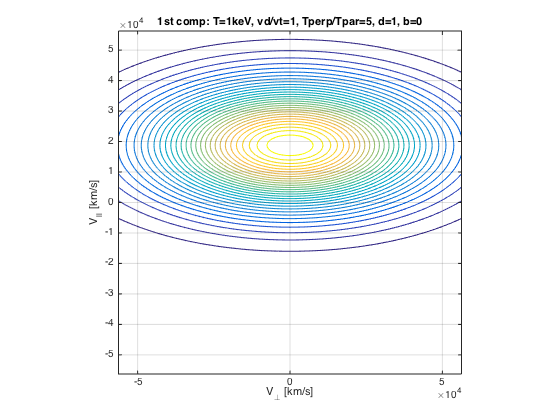
\includegraphics[width=.7\linewidth]{f_whamp_Ex1}
%\centering
\caption{Example distribution function. Drift velocity $v_d=v_{th}$ and temperature
anisotropy is such that $\Tp/\Tz=2$. The MATLAB commands below are used to create the plot.
}
\label{fig:f_ex1}
  \end{center}
\begin{verbatim}
Electrons = struct('m',0,'n',1,'t',1,'a',5,'vd',1,'d',1,'b',0);
whamp.plot_f(Electrons,'km/s')
\end{verbatim}
\end{figure}

\newpage
\section{\WHAMP, running code}
\subsection{Running from terminal}
Plasma model is specified with an input file. Note that $a=\ga_1, b=\ga_2$
\begin{verbatim}
============ Model files ===========
n(1)  n(2)  ...  n(10)   /per m3/
t(1)  t(2)  ...  t(10)   / keV, T_par /
d(1)  d(2)  ...  d(10)   / loss cone parameter, default 1.0 (no loss cone) /
a(1)  a(2)  ...  a(10)   / t_perp/t_par, default 1.0 /
b(1)  b(2)  ...  b(10)   / default 0, i.e. no loss cone/
ass(1)  ass(2)  ...  ass(10)    / 0-electrons, 1-protons, 16-oxygen /
vd(1)  vd(2)  ...  vd(10)   / v_drift/v_term /
fce / electron gyrofrequency in kHz /
pzl     / 1 - log scale, 0 - linear scale /

=====================================
Plasma with B=100nT, n=1cm-3, there are only
oxygen ions (Tperp=50eV, Tpar=10eV, vd=1*vt_par)
and 1eV electrons.
============ Example file with 9 lines ===========
1.e6 1.e6 0.0 0.0 0.0 0.0 0.0 0.0 0.0 0.0
.001 .001 0.0 0.0 0.0 0.0 0.0 0.0 0.0 0.0
1.   1.   1.0 1.0 1.0 1.0 1.0 1.0 1.0 1.0
5.   1.   1.0 1.0 1.0 1.0 1.0 1.0 1.0 1.0
0.0  0.0  0.0 0.0 0.0 0.0 0.0 0.0 0.0 0.0
16.  0.0  0.0 0.0 0.0 0.0 0.0 0.0 0.0 0.0
1.   0.0  0.0 0.0 0.0 0.0 0.0 0.0 0.0 0.0
2.8
0

\end{verbatim}

Plasma parameters can be also changed later during the running of the code.

To start the WHAMP just execute:
\\\texttt{>whamp -file <modelfile>}

A real example that can be run from \texttt{src} directory:
\begin{verbatim}
> ./whamp -file ../Models/Ex1
# PLASMA FREQ.:     8.9786KHZ GYRO FREQ.:    2.8000KHZ   ELECTRON DENSITY:1.00000E+06M-3
# O+   DN= 1.00000E+06  T=  0.01000  D=1.00  A=5.00  B=0.00 VD= 1.00
# e-   DN= 1.00000E+06  T=  0.00100  D=1.00  A=1.00  B=0.00 VD= 0.00
#INPUT:
\end{verbatim}

You can get help for input by entering "h". You get
\begin{verbatim}
 AN INPUT LINE MAY CONSIST OF UP TO 80 CHARACTERS.
 THE FORMAT IS:
 NAME1=V11,V12,V13,...NAME2=V21,V22,...NAME
 THE NAMES ARE CHOSEN FROM THE LIST:

 NAME              PARAMETER
 A(I)              THE ALPHA1 PARAMETER IN THE DISTRIBUTION.
                   (I) IS THE COMPONENT NUMBER, I=1 - 6.
 B(I)              THE ALPHA2 PARAMETER IN THE DISTRIBUTION.
 C                 THE ELECTRON CYCLOTRON FREQ. IN KHZ.
 D(I)              THE DELTA PARAMETER IN THE DISTRIBUTION
 F                 FREQUENCY, START VALUE FOR ITERATION.
 L            L=1  THE P AND Z PARAMETERS ARE INTERPRETED
                   AS LOGARITHMS OF THE WAVE NUMBERS. THIS
                   OPTION ALLOWS FOR LOGARITHMIC STEPS.
              L=0  DEFAULT VALUE. LINEAR STEPS.
 M(I)              MASS IN UNITS OF PROTON MASS.
 N(I)              NUMBER DENSITY IN PART./CUBIC METER
 P(I)              PERPENDICULAR WAVE VECTOR COMPONENTS.
                   P(1) IS THE SMALLEST VALUE, P(2) THE
                   LARGEST VALUE, AND P(3) THE INCREMENT.
 S                 STOP! TERMINATES THE PROGRAM.
 T(I)              TEMPERATURE IN KEV
 V(I)              DRIFT VELOCITY / THERMAL VELOCITY.
 Z(I)              Z-COMPONENT OF WAVE VECTOR. I HAS THE
                   SAME MEANING AS FOR P(I).
 A NAME WITHOUT INDEX REFERS TO THE FIRST ELEMENT, "A" IS
 THUS EQUIVALENT TO "A(1)". THE VALUES V11,V12,.. MAY BE
 SPECIFIED IN I-, F-, OR E-FORMAT, SEPARATED BY COMMA(,).
 THE "=" IS OPTIONAL, BUT MAKES THE INPUT MORE READABLE.
 EXAMPLE: INPUT:A1.,2. B(3).5,P=.1,.2,1.E-2
 THIS SETS A(1)=1., A(2)=2., B(3)=.5, P(1)=.1, P(2)=.2,
 AND P(3)=.01. IF THE INCREMENT P(3)/Z(3) IS NEGATIVE, P/Z
 WILL FIRST BE SET TO P(2)/Z(2) AND THEN STEPPED DOWN TO
 P(1)/Z(1)
 THE LAST SPECIFIED OF P AND Z WILL VARY FIRST.
 IF THE LETTER "O" (WITHOUT VALUE) IS INCLUDED, YOU WILL
  BE ASKED TO SPECIFY A NEW OUTPUT FORMAT.

\end{verbatim}

\subsection{\WHAMP\ running from matlab}
See help where are given examples: 

\texttt{help whamp.run}

\subsection{\WHAMP\ input}
Plasma parameters can be specified in the model file. To start the calculations the range of $\kp$ and $\kz$, the step length in $\kp$ and \kz, and a start value for the frequency must be specified. When running \WHAMP, this means specifying $p,z$ and $f$, where $p=\kappa_\perp^1=\kp V_{th}^1/\Om^1, z=\kappa_\parallel^1=\kz V_{th}^1/\Om^1, f=\w/\Om^1$, where the thermal velocity of plasma with temperature $T^{eV}$ (expressed in eV) can be calculated as $V_{th}=\sqrt{2 e T^{eV}/m}$. \textbf{The normalization is always with respect to the first component of the plasma model}. In an anisotropic plasma it is the parallel thermal speed that is used for thermal velocity estimates. 
Using frequency in Hz instead of rad/s we have
\eql{pzf}{\text{p}=\frac{V_{th}^1}{\lambda_\perp f_{c1}}, \quad
        \text{z}=\frac{V_{th}^1}{\lambda_\parallel f_{c1}}, \quad
        \text{f}=\frac{\w}{f_{c1}}.}

In our example file $O^+$ is the first component. The gyrofrequency of $O^+$ is 0.095~Hz, the thermal speed of 10eV oxygen ions is 10.9~km/s. The \Alfven\ velocity is 545~km/s. Thus if we with WHAMP want to find \Alfven\ wave below oxygen gyrofrequency, let's say at 0.01~Hz, we would put $p=0$ (parallel propagation), $f=f^{Hz}/f_{cO^+}=0.01/.095\approx 0.105$, and parallel wavelength $\lambda=v_A/f=0.545\ 10^6/0.0105=51.9\ 10^6$~km and $z=10.9\ 10^3/(51.9\  10^6*0.095)\approx 0.0022$. Running \WHAMP\ from terminal we would enter:

\begin{verbatim}
p0z.0022f.1
\end{verbatim}

\subsection{\WHAMP\ output when running from terminal}
\WHAMP\ can print different output parameters. The simplest is to print wave vectors and frequency, for this enter "pzf". The output has the same normalization as input. The example above would be:

\begin{verbatim}
> ./whamp -file ../Models/Ex1
# PLASMA FREQ.:     8.9786KHZ GYRO FREQ.:    2.8000KHZ   ELECTRON DENSITY:1.00000E+06M-3
# O+   DN= 1.00000E+06  T=  0.01000  D=1.00  A=5.00  B=0.00 VD= 1.00
# e-   DN= 1.00000E+06  T=  0.00100  D=1.00  A=1.00  B=0.00 VD= 0.00
#INPUT:

p0z.0022f.1
#OUTPUT:

pzf
    0.0000000      0.0022000    1.0640799E-01  3.34E-11

#INPUT:
\end{verbatim}

NOTE! For the frequency both, the real and imaginary part is printed.

The following options are available for output

\begin{verbatim}
####
============ output ===========

    e   (ex,ey,ez)
    b   (bx,by,bz)
    f   frequency <real,imaginery>
    g   group velocity
    h   |e|/|b| [(mV/m)/nT]
    p   k perpendicular
    s   (sp, sz)   spatial growth
    u   energy ration between the total wave energy and energy in electric field
    v   Poynting flux (in uW/m2 for <E^2>=0.5(mV/m)^2)
    z   k paralel
    y   energy density and flux of each component

\end{verbatim}

Thus if you would like to print k-vector components and frequency, and in the next line all electric field components, you would enter "pzf/e". Example from session:

\begin{verbatim}
#INPUT:

o
#OUTPUT:

pzf/e
    0.0000000      0.0022000    1.0640799E-01  3.34E-11
 EX= 0.7071  0.0000  EY=-0.0000  0.7071  EZ= 0.0000  0.0000

#INPUT:

\end{verbatim}

For fields the first is real and the second is imaginary part. Note that in this example the wave is right hand polarized $E_y=iE_x$.

\subsection{Dispersion surfaces}

One can specify input of wave vectors and steps in log$_{10}$ space executing "l1" in terminal. This is convenient when estimating dispersion surfaces over large wave vector interval. Let's look at the interval $p=10^{-3}\ldots 10^{-1},z=10^{-3}\ldots 10^{-1}$, where we for every $p$ value go through all $z$ values ($z$ changes first). First we find the starting point, then we check $z$ interval for only one $p$ value and finally we run $p$ intervals for different $z$ values.

\begin{verbatim}
#INPUT:

l1
    0.0010000      0.0010000    4.7821169E-02 -3.90E-08

#INPUT:

z-3p-3f.04
    0.0010000      0.0010000    4.7821169E-02 -3.90E-08

#INPUT:

z-3,-1,.3
    0.0010000      0.0010000    4.7821169E-02 -3.90E-08
    0.0010000      0.0019953    9.9003895E-02 -2.69E-08
    0.0010000      0.0039811    2.1508729E-01 -6.39E-08
    0.0010000      0.0079433    4.7770868E-01 -3.44E-08
    0.0010000      0.0158489    1.1588537E+00 -2.81E-08
    0.0010000      0.0316228    3.2487234E+00 -2.59E-08
    0.0010000      0.0630957    1.0804231E+01 -1.43E-09

#INPUT:

z-3,-1,.3p-3,-1,.3

\end{verbatim}

After the last command one gets the screen full with the result. These results one can copy into some file "test" which one can load in from matlab and plot as a dispersion surface. The command lines in matlab are

\begin{verbatim}
load test
[p,z,f,fim]=whamp.m2xyz(test);
surf(log10(p),log10(z),f)
xlabel('p');ylabel('z');zlabel('f');
\end{verbatim}

\texttt{whamp.m2xyz} reorders the \WHAMP\ result file into $p,z$ vectors and $f,\gamma$ matrices.

\begin{figure}[htb]
  \begin{center}
    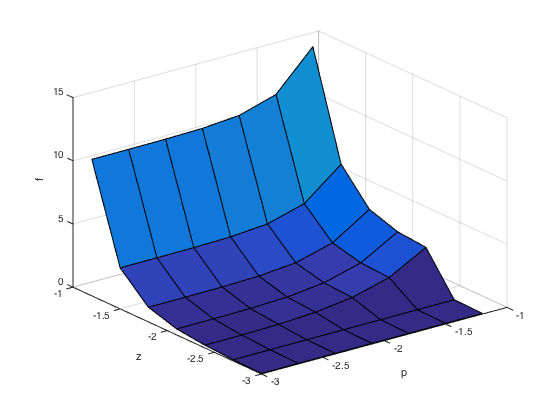
\includegraphics[width=.7\linewidth]{disp_surf_Ex1}
  \end{center}
\centering
\label{fig:disp}
\end{figure}

The result is OK for the first \WHAMP\ try but one can note a few things
\begin{itemize}
    \item One needs smaller steps to get nice dispersion relation,
    \item One can jump from one dispersion surface to another, \WHAMP\ tries to find the closest one from some given initial conditions which often does not mean the same as to stay on the same dispersion surface.
    \item One can expect a lot of "trial and error" before one gets a satisfactory result
   \end{itemize}

Constructing the same dispersion surface from MATLAB would be: 
\begin{verbatim}
Oxygen              = struct('m',16,'n',1,'t',10,'a',5,'vd',1);
Electrons           = struct('m',0,'n',1,'t',1);
PlasmaModel         = struct('B',100);
PlasmaModel.Species = {Oxygen,Electrons};
InputParameters     = struct('fstart',0.04,'kperp',[-3 .3 -1],...
                      'kpar',[-3 .3 -1],'useLog',1);
Output              = whamp.run(PlasmaModel,InputParameters)

surf(log10(Output.kperp),log10(Output.kpar),real(Output.f))
xlabel('p');
ylabel('z');
zlabel('f');
\end{verbatim}

%\subsection{Analytic tests}
%Here we show some example dispersion relations and expected damping/growth rates for some parameters where relatively precise analytic solutions exist. 
%
%We introduce more non-dimensional parameters 
%\begin{gather}
% \tilde{\omega}^j=\tilde{kappa}_{\bot}^{j}=\frac{k_{\bot}\cdot V_{th}^{j}}{\Omega^{j}} \; ; \;\;\;
% \kappa _{\|}^{j}=\frac{k_{\|}\cdot V_{th}^{j}}{\Omega^{j}}     \; ; \;\;\;
% \tilde{\omega}_{pl}^{j}=\frac{\omega _{pl}}{\Omega^{j}} \; ; \;
% \tilde{\omega}^{j}=\frac{\omega}{\Omega^{j}}  \; ; \;
% \tilde{c}=\frac{c}{V_{th}^{1}}
%\end{gather}


\subsection{References}
\begin{itemize}
\item WHAMP - latest version on \url{https://github.com/irfu/whamp}
\end{itemize}
\vspace{2cm}

\centering
Good luck!

\end{document}



